% LuaLaTeX文書; 文字コードはUTF-8
\documentclass[unicode,12pt]{beamer}% 'unicode'が必要
\usepackage{luatexja}% 日本語したい
\usepackage[ipaex]{luatexja-preset}% IPAexフォントしたい
\renewcommand{\kanjifamilydefault}{\gtdefault}% 既定をゴシック体に
\usepackage{tikz}
\usepackage{ytableau}
\usetikzlibrary{intersections, calc, arrows.meta}

% あとは欧文の場合と同じ
\usetheme{Copenhagen}
\setbeamertemplate{theorems}[numbered]
\theoremstyle{definition}
\newtheorem{defin}{定義}[section]
\newtheorem{theo}[defin]{定理}
\newtheorem{cor}[defin]{系}
\newtheorem{prop}[defin]{命題}
\newtheorem{lemm}[defin]{補題}
\newtheorem{notice}[defin]{注意}
\theoremstyle{example}
\newtheorem{eg}[defin]{例}
\newtheorem{conj}[defin]{予想}

\newcommand{\integer}{\mathbb{Z}}
\newcommand{\complex}{\mathbb{C}}
\newcommand{\set}[2]{\left\{\:#1\:\middle|\:#2\:\right\}}
\newcommand{\codim}[1]{\text{codim}\:#1}



\title{同変シューベルト計算\\における組合せ論}
\author{赤松輝海}
\date{令和7年2月3日}
\institute{京都大学大学院理学研究科数学・数理解析専攻修士課程}


\begin{document}

%1
\begin{frame}
  \titlepage
\end{frame}

%2
\begin{frame}{概要}
  $2$つのSchubert類の積を展開したときの係数はLittlewood-Richardson数と呼ばれ,その計算アルゴリズムがいくつも知られている.同変コホモロジーにおいてもSchubert多様体は同変コホモロジー環の基底を定める.このときの構造定数,すなわち,$S_\lambda$を同変Schubert類とし,
  \[
  S_\lambda S_\mu = \sum_{\nu\in\binom{n}{k}}C^\nu_{\lambda\mu}S_\nu,\quad C^\nu_{\lambda\mu}\in\integer[y_1,\cdots,y_n]
  \]
  としたときの多項式$C^\nu_{\lambda\mu}$を同変Littlewood-Richardson係数と呼ぶ.
\end{frame}

%3
\begin{frame}{概要}
  本発表では$C^\nu_{\lambda\mu}$を計算する組合せ論的対象として
  \begin{enumerate}
    \item Knutson-Taoによるpuzzle
    \item Thomas-Yongによるedge labeled tableaux
  \end{enumerate}
  を紹介し,その同値性について解説する.
\end{frame}

%4
\begin{frame}{目次}
  \tableofcontents
\end{frame}




\section[]{同変Schubert類}

%6
\begin{frame}{同変Schubert類}
  $\text{Gr}_k(\complex^n)=\set{V\subset\complex^n}{\dim V = k}$とする.
  $\binom{n}{k}$を$0$と$1$からなる文字列で,$k$個の$1$を含んでいるようなもの全体とする.$\lambda\in\binom{n}{k}$に対して
  \[
  \Omega_\lambda = \set{V\in \text{Gr}_k(\complex^n)}{\dim V\cap F^i \geq \dim \complex^\lambda\cap F^i}
  \]
  をSchubert多様体という.ここで$F^i = \langle e_{n-i+1},\cdots,e_n \rangle$,$\complex^\lambda = \langle \lambda_1e_1,\cdots,\lambda_ne_n \rangle$.$|\lambda| = \#\set{(i, j)}{\lambda_i = 1,\lambda_j = 0, i < j}$とすると$\codim\Omega_\lambda=|\lambda|$である.
\end{frame}

%7
\begin{frame}{同変Schubert類}
  $T=(\complex^\times)^n$は自然に$\text{Gr}_k(\complex^n)$に作用し$\Omega_\lambda$は$T$不変.
  通常のコホモロジーと同様$\Omega_\lambda$は$2|\lambda|$次の同変コホモロジー類を定める.これを$S_\lambda$と置き,同変Schubert類と呼ぶ.
  \begin{prop}\label{basis theorem}
    $\{S_\lambda\}_{\lambda\in\binom{n}{k}}$は$H^*_T(\text{Gr}_k(\complex^n))$の$H^*_T(\text{pt})\simeq\integer[y_1,\cdots,y_n]$上の基底をなす.
  \end{prop}
  命題\ref{basis theorem}より,
  \[
    S_\lambda S_\mu = \sum_{\nu\in\binom{n}{k}}C^\nu_{\lambda\mu}S_\nu,\quad C^\nu_{\lambda\mu}\in\integer[y_1,\cdots,y_n]
  \]
  と表した時の$C^\nu_{\lambda\mu}$を同変Littlewood-Richardson係数と呼ぶ.
\end{frame}

\section[]{puzzleによる方法}

%8
\begin{frame}{puzzleによる方法}
  \begin{defin}[puzzle]
    以下の$8$種類の図形をpuzzle pieceと言い,これらを組み合わせて得られる正三角形をpuzzleと呼ぶ.
  \begin{figure}[htbp]
    \centering
    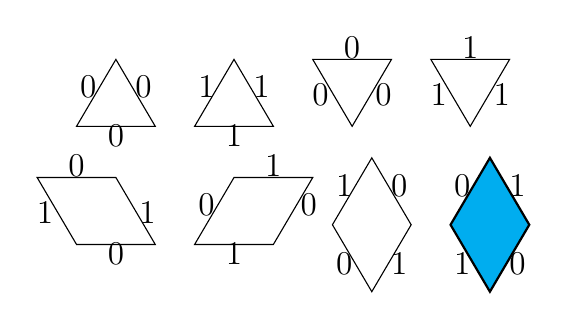
\begin{tikzpicture}[xscale=0.5,yscale=0.5]
      \coordinate (A) at (0,0);
      \coordinate (B) at (2,0);
      \coordinate (C) at (1,1.7);

      \draw (A)--(B)--(C)--cycle;
      \node[font=\large] at ($(A)+(1,-0.25)$) {$0$};
      \node[font=\large] at ($(A)+(0.3,1)$) {$0$};
      \node[font=\large] at ($(A)+(1.7,1)$) {$0$};

      \coordinate(P) at (3,0);
      \draw ($(A)+(P)$)--($(B)+(P)$)--($(C)+(P)$)--cycle;
      \node[font=\large] at ($(P)+(1,-0.25)$) {$1$};
      \node[font=\large] at ($(P)+(0.3,1)$) {$1$};
      \node[font=\large] at ($(P)+(1.7,1)$) {$1$};

      \coordinate (Q) at (6,0);
      \draw ($(A)+(Q)+(0,1.7)$)--($(B)+(Q)+(0,1.7)$)--($(C)+(Q)-(0,1.7)$)--cycle;
      \node[font=\large] at ($(Q)+(0.2,0.8)$) {$0$};
      \node[font=\large] at ($(Q)+(1.8,0.8)$) {$0$};
      \node[font=\large] at ($(Q)+(1,2)$) {$0$};

      \coordinate (R) at (9,0);
      \draw ($(A)+(R)+(0,1.7)$)--($(B)+(R)+(0,1.7)$)--($(C)+(R)-(0,1.7)$)--cycle;
      \node[font=\large] at ($(R)+(0.2,0.8)$) {$1$};
      \node[font=\large] at ($(R)+(1.8,0.8)$) {$1$};
      \node[font=\large] at ($(R)+(1,2)$) {$1$};

      \draw ($(A)-(0,3)$)--($(B)-(0,3)$)--($(C)-(0,3)$)--($(C)-(2,3)$)--cycle; 
      \node[font=\large] at ($(A)+(1,-3.25)$) {$0$};
      \node[font=\large] at ($(A)+(1.8,-2.2)$) {$1$};
      \node[font=\large] at ($(A)+(-0.8,-2.2)$) {$1$};
      \node[font=\large] at ($(A)+(0,-1)$) {$0$};

      \draw ($(A)-(-3,3)$)--($(B)-(-3,3)$)--($(C)-(-5,3)$)--($(C)-(-3,3)$)--cycle;
      \node[font=\large] at ($(P)+(1,-3.25)$) {$1$};
      \node[font=\large] at ($(P)+(2.9,-2)$) {$0$};
      \node[font=\large] at ($(P)+(0.3,-2)$) {$0$};
      \node[font=\large] at ($(P)+(2,-1)$) {$1$}; 

      \draw ($(A)+(6.5,-2.5)$)--($(C)+(6.5,-2.5)$)--($(B)+(6.5,-2.5)$)--($(C)+(6.5,-5.9)$)--cycle;
      \node[font=\large] at ($(Q)+(0.8,-1.5)$) {$1$};
      \node[font=\large] at ($(Q)+(2.2,-1.5)$) {$0$};
      \node[font=\large] at ($(Q)+(2.2,-3.5)$) {$1$};
      \node[font=\large] at ($(Q)+(0.8,-3.5)$) {$0$};

      \fill[cyan] ($(A)+(9.5,-2.5)$)--($(C)+(9.5,-2.5)$)--($(B)+(9.5,-2.5)$)--($(C)+(9.5,-5.9)$)--cycle;
      \draw[thick] ($(A)+(9.5,-2.5)$)--($(C)+(9.5,-2.5)$)--($(B)+(9.5,-2.5)$)--($(C)+(9.5,-5.9)$)--cycle;
      \node[font=\large] at ($(R)+(0.8,-1.5)$) {$0$};
      \node[font=\large] at ($(R)+(2.2,-1.5)$) {$1$};
      \node[font=\large] at ($(R)+(2.2,-3.5)$) {$0$};
      \node[font=\large] at ($(R)+(0.8,-3.5)$) {$1$};
    \end{tikzpicture}
  \end{figure}
  青塗された図形をequivariant pieceという.
  \end{defin}
\end{frame}

%9
\begin{frame}{puzzleによる方法}
  \begin{eg}
    puzzleの例.
    \begin{figure}[htbp]
      \centering
      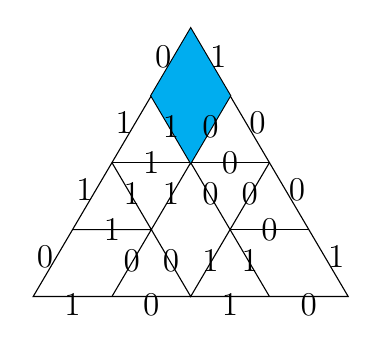
\begin{tikzpicture}[xscale=0.5,yscale=0.5]
        \draw (0,0)--(8,0)--(4,6.8)--cycle;
        \draw (2,0)--(3,1.7)--(1,1.7);
        \draw (3,1.7)--(4,0)--(5,1.7)--(6,0);
        \draw (5,1.7)--(7,1.7);
  
        \draw (2,3.4)--(3,1.7)--(4,3.4)--(5,1.7)--(6,3.4);
        \draw (2,3.4)--(6,3.4);
  
        \draw[thick] (3,5.1)--(4,3.4)--(5,5.1)--(4,6.8)--cycle;
        \fill[cyan] (3,5.1)--(4,3.4)--(5,5.1)--(4,6.8)--cycle;
  
        \node[font=\large] at (1,-0.2) {$1$};
        \node[font=\large] at (3,-0.2) {$0$};
        \node[font=\large] at (5,-0.2) {$1$};
        \node[font=\large] at (7,-0.2) {$0$};
  
        \node[font=\large] at (2,1.7) {$1$};
        \node[font=\large] at (6,1.7) {$0$};
  
        \node[font=\large] at (3,3.4) {$1$};
        \node[font=\large] at (5,3.4) {$0$};
  
  
        \coordinate (A) at (0.3, 1);
        \coordinate (P) at (1,1.7);
        \node[font=\large] at (A) {$0$};
        \node[font=\large] at ($(A)+(P)$) {$1$};
        \node[font=\large] at ($(A)+2*(P)$) {$1$};
        \node[font=\large] at ($(A)+3*(P)$) {$0$};
  
        \coordinate (B) at (7.7, 1);
        \coordinate (Q) at (-1,1.7);
        \node[font=\large] at (B) {$1$};
        \node[font=\large] at ($(B) + (Q)$) {$0$};
        \node[font=\large] at ($(B) + 2*(Q)$) {$0$};
        \node[font=\large] at ($(B) + 3*(Q)$) {$1$};
  
        \node[font=\large] at (2.5,0.9) {$0$};
        \node[font=\large] at (3.5,0.9) {$0$};
        \node[font=\large] at (4.5,0.9) {$1$};
        \node[font=\large] at (5.5,0.9) {$1$};
        
        \node[font=\large] at (2.5,2.6) {$1$};
        \node[font=\large] at (3.5,2.6) {$1$};
        \node[font=\large] at (4.5,2.6) {$0$};
        \node[font=\large] at (5.5,2.6) {$0$};
  
        \node[font=\large] at (3.5,4.3) {$1$};
        \node[font=\large] at (4.5,4.3) {$0$};
      \end{tikzpicture}
    \end{figure}
  \end{eg}
\end{frame}

%10
\begin{frame}{puzzleによる方法}
  \begin{defin}
    puzzle $P$に対して,$P$の周の各辺上の文字を図の方向に読んで得られる文字列をそれぞれ$\lambda,\mu,\nu$とするとき,$\partial P = \Delta^\nu_{\lambda\mu}$と書く.

  \begin{figure}
    \center
    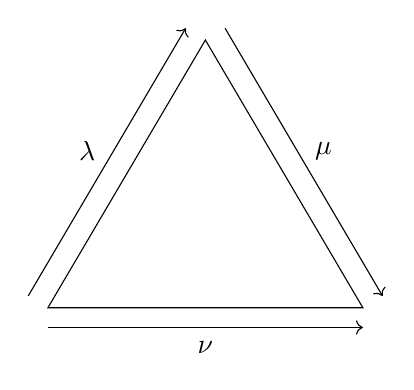
\begin{tikzpicture}[xscale=0.5,yscale=0.5]
      \begin{scope}
        \draw (0,0)--(8,0)--(4,6.8)--cycle;
        \draw[->] (-0.5,0.3) -- ++(4,6.8);
        \node at (2-1,3.4+0.58) {$\lambda$};

        \draw[->] (4+0.5,6.8+0.3) -- ++(4,-6.8);
        \node at (6+1,3.4+0.58) {$\mu$};

        \draw[->] (0,-0.5) -- (8,-0.5);
        \node at (4,-1) {$\nu$};
      \end{scope}
      \begin{scope}
        
      \end{scope}
    \end{tikzpicture}
  \end{figure}
  \end{defin}
\end{frame}

%11
\begin{frame}{puzzleによる方法}
  \begin{eg}
    puzzleの例.
    \begin{figure}[htbp]
      \centering
      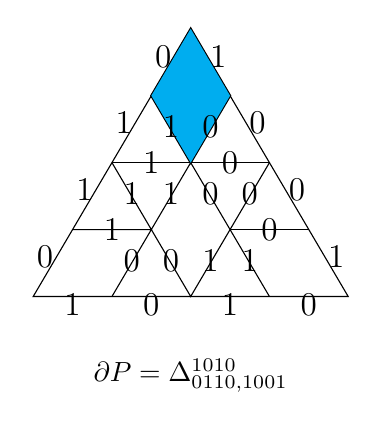
\begin{tikzpicture}[xscale=0.5,yscale=0.5]
        \draw (0,0)--(8,0)--(4,6.8)--cycle;
        \draw (2,0)--(3,1.7)--(1,1.7);
        \draw (3,1.7)--(4,0)--(5,1.7)--(6,0);
        \draw (5,1.7)--(7,1.7);
  
        \draw (2,3.4)--(3,1.7)--(4,3.4)--(5,1.7)--(6,3.4);
        \draw (2,3.4)--(6,3.4);
  
        \draw[thick] (3,5.1)--(4,3.4)--(5,5.1)--(4,6.8)--cycle;
        \fill[cyan] (3,5.1)--(4,3.4)--(5,5.1)--(4,6.8)--cycle;
  
        \node[font=\large] at (1,-0.2) {$1$};
        \node[font=\large] at (3,-0.2) {$0$};
        \node[font=\large] at (5,-0.2) {$1$};
        \node[font=\large] at (7,-0.2) {$0$};
  
        \node[font=\large] at (2,1.7) {$1$};
        \node[font=\large] at (6,1.7) {$0$};
  
        \node[font=\large] at (3,3.4) {$1$};
        \node[font=\large] at (5,3.4) {$0$};
  
  
        \coordinate (A) at (0.3, 1);
        \coordinate (P) at (1,1.7);
        \node[font=\large] at (A) {$0$};
        \node[font=\large] at ($(A)+(P)$) {$1$};
        \node[font=\large] at ($(A)+2*(P)$) {$1$};
        \node[font=\large] at ($(A)+3*(P)$) {$0$};
  
        \coordinate (B) at (7.7, 1);
        \coordinate (Q) at (-1,1.7);
        \node[font=\large] at (B) {$1$};
        \node[font=\large] at ($(B) + (Q)$) {$0$};
        \node[font=\large] at ($(B) + 2*(Q)$) {$0$};
        \node[font=\large] at ($(B) + 3*(Q)$) {$1$};
  
        \node[font=\large] at (2.5,0.9) {$0$};
        \node[font=\large] at (3.5,0.9) {$0$};
        \node[font=\large] at (4.5,0.9) {$1$};
        \node[font=\large] at (5.5,0.9) {$1$};
        
        \node[font=\large] at (2.5,2.6) {$1$};
        \node[font=\large] at (3.5,2.6) {$1$};
        \node[font=\large] at (4.5,2.6) {$0$};
        \node[font=\large] at (5.5,2.6) {$0$};
  
        \node[font=\large] at (3.5,4.3) {$1$};
        \node[font=\large] at (4.5,4.3) {$0$};

        \node at (4,-2) {$\partial P = \Delta^{1010}_{0110,1001}$};
      \end{tikzpicture}
    \end{figure}
  \end{eg}
\end{frame}

%12
\begin{frame}{puzzleによる方法}
  \begin{defin}[puzzleのweight]
    $p$をpuzzle $P$のequivariant pieceとする.図のように$p$から線分を引いたときの$P$の下辺との交点の位置によって$\text{wt}(p)\in\integer[y_1,\cdots,y_n]$を定義する.
  \begin{figure}[htbp]
    \centering
    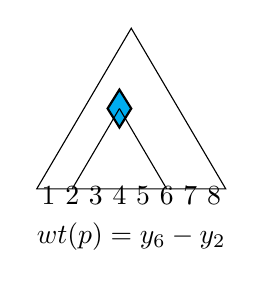
\begin{tikzpicture}[xscale=0.3,yscale=0.3]
      \draw (0,0)--(8,0)--(4,6.8)--cycle;
      \fill[cyan] (3,3.4)--(3.5,2.6)--(4,3.4)--(3.5,4.2)--cycle;
      \draw[thick] (3,3.4)--(3.5,2.6)--(4,3.4)--(3.5,4.2)--cycle;
      
      \draw (3.5,3.4)--(1.5,0);
      \draw (3.5,3.4)--(5.5,0);
  
  
      \node at (0.5,-0.3) {$1$};
      \node at (1.5,-0.3) {$2$};
      \node at (2.5,-0.3) {$3$};
      \node at (3.5,-0.3) {$4$};
      \node at (4.5,-0.3) {$5$};
      \node at (5.5,-0.3) {$6$};
      \node at (6.5,-0.3) {$7$};
      \node at (7.5,-0.3) {$8$};

      \node at (4,-2) {$\text{wt}(p)=y_6-y_2$};
    \end{tikzpicture}
  \end{figure}
  また,$\text{wt}(P) = \prod_{p}\text{wt}(p)$とする.
  \end{defin}
\end{frame}

%13
\begin{frame}{puzzleによる方法}
  \begin{theo}[Knutson-Tao]
    同変Littlewood-Richardson係数$C^\nu_{\lambda\mu}$について
    \[
    C^\nu_{\lambda\mu} = \sum_{\partial P = \Delta^\nu_{\lambda\mu}}\text{wt}(P)
    \]
    が成り立つ.
  \end{theo}
\end{frame}

\section[]{edge labeled tableauxによる方法}

%14
\begin{frame}{edge labeled tableauxによる方法}
  $\lambda\in\binom{n}{k}$を左から読んで$i_1<\cdots<i_k$番目に$1$が現れるとする.
  \[
  l_a = \#\set{j}{j > i_a, \lambda_j = 0},\quad \text{for }a = 1,\cdots,k
  \]
  によって分割$l=(l_1,\cdots,l_k)$が得られる.この対応によって$\binom{n}{k}$は$((n-k)^k)$に含まれる分割と同一視できる.
  \begin{figure}
    \center
    \begin{tikzpicture}
      \node at (0,0) {$\lambda = 10010$};
      \node at (1.5,0) {$\rightarrow$};

      \begin{scope}[xshift = 2.7cm, yshift = 0.8cm]
        \node at (-0.4,-0.8) {$l=$};
        \draw (0,0) -- ++(2.4,0);
        \draw (0,-0.8) -- ++(2.4,0);
        \draw (0,-1.6) -- ++(0.8,0);
        \draw (0,0) -- ++(0,-1.6);
        \draw (0.8,0) -- ++(0,-1.6); 
        \draw (1.6,0)-- ++(0,-0.8);
        \draw (2.4,0)-- ++(0,-0.8);
      \end{scope}
    \end{tikzpicture}
  \end{figure}
\end{frame}

%15
\begin{frame}{edge labeled tableauxによる方法}
  \begin{defin}[equivariant filling]
    分割$\lambda, \nu$に対して,$\lambda_i\leq\nu_i$がすべての$i$で成り立つとき,$\lambda\leq\nu$とする.このとき$\nu$の箱であって$\lambda$の箱でないもの全体を歪Young図形といい$\nu/\lambda$と書く.

  $\nu/\lambda$の各箱に$1$から$m$までの数字を$1$つ書き入れ,$\lambda$のよりも下にある水平方向の各辺に$\{1,\cdots,m\}$の空でもよい部分集合を書き入れたものをequivariant fillingという.
  \end{defin}
\end{frame}

%16
\begin{frame}{edge labeled tableauxによる方法}
  \footnotesize
  \begin{defin}[equivariant standard tableaux]
    形が$\nu/\lambda$のequivariant fillingのうち,次の条件を満たすものをequivariant standard tableauxという.
  \begin{itemize}
    \item $1$から$m$までの各数字が,いずれかの箱のラベルに現れるか,またはいずれかの辺のラベルの要素になっている.また$1$から$m$までの各数字がちょうど1回現れる.
    \item 各箱のラベルについて,左隣の箱のラベルよりも大きい.
    \item 各箱のラベルについて,上辺のラベルが空でないなら,その最大値よりも大きい.空であるならば,すぐ上の箱のラベルより大きい.
    \item 各辺のラベルについて,そのすべての数字がすぐ上の箱に書かれたラベルよりも大きい.
  \end{itemize}
  形が$\nu/\lambda$で$1$から$m$までの数字が書かれたequivariant standard tableauxの全体の集合を$\text{EqSYT}(\nu/\lambda, m)$とする.
  \end{defin}
  \normalsize
\end{frame}

%17
\begin{frame}{edge labeled tableauxによる方法}
  \begin{eg}
    equivariant standard tableauxとそうでないものの例.左図は$\{3,5\}$が$\lambda=(2,2,1)$の境界から下にないためequivariant fillingでない.中央の図は$1$と$2$が$\lambda=(1,1,1)$の境界から下にないためequivariant fillingでない.右図は$(4,4,2)/(3,3,1)$上のequivariant standard tableauxの例である.
  \begin{figure}
    \centering
    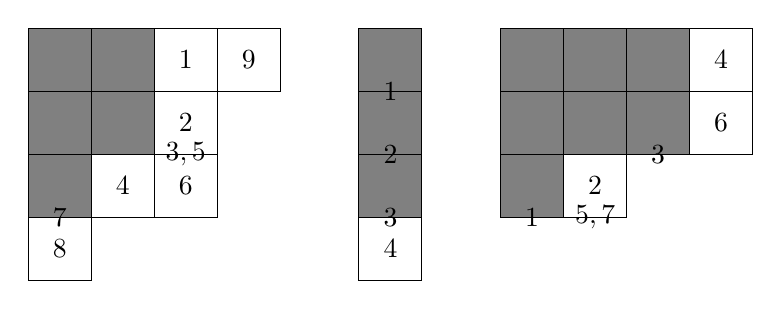
\begin{tikzpicture}
      \begin{scope}
        \fill[gray] (0,0)--(1.6,0)--(1.6,-1.6)--(0.8,-1.6)--(0.8,-2.4)--(0,-2.4)--cycle;
        \draw (0,0)--(0,-3.2)--(0.8,-3.2)--(0.8,-2.4)--(2.4,-2.4)--(2.4,-0.8)--(3.2,-0.8)--(3.2,0)--cycle;
        \draw (0,-0.8)--(2.4,-0.8);
        \draw (0,-1.6)--(2.4,-1.6);
        \draw (0,-2.4)--(0.8,-2.4);
        \draw (0.8,0)--(0.8,-2.4);
        \draw (1.6,0)--(1.6,-2.4);
        \draw (2.4,0)--(2.4,-0.8);
  
        \node at (2,-0.4) {$1$};
        \node at (2.8,-0.4) {$9$};
        \node at (2,-1.2) {$2$};
        \node at (1.2,-2) {$4$};
        \node at (2,-2) {$6$};
        \node at (0.4,-2.8) {$8$};
  
        \node at (0.4,-2.4) {$7$};
        \node at (2,-1.6) {$3,5$};
      \end{scope}
      \begin{scope}[xshift=4.2cm]
        \fill[gray] (0,0) rectangle ++(0.8,-2.4);
        \draw (0,0) rectangle ++(0.8,-3.2);
        \draw (0,-0.8) -- ++(0.8,0);
        \draw (0,-1.6) -- ++(0.8,0);
        \draw (0,-2.4) -- ++(0.8,0);
        
        \node at (0.4,-0.8) {$1$};
        \node at (0.4,-1.6) {$2$};
        \node at (0.4,-2.4) {$3$};
        \node at (0.4,-2.8) {$4$};
      \end{scope}
      \begin{scope}[xshift=6cm]
        \fill[gray] (0,0)--(2.4,0)--(2.4,-1.6)--(0.8,-1.6)--(0.8,-2.4)--(0,-2.4)--cycle;
        \draw (0,0)--(3.2,0)--(3.2,-1.6)--(1.6,-1.6)--(1.6,-2.4)--(0,-2.4)--cycle;
        \draw (0.8,0)-- +(0,-2.4);
        \draw (1.6,0)-- +(0,-1.6);
        \draw (2.4,0)-- +(0,-1.6);
        \draw (0,-0.8)-- +(3.2,0);
        \draw (0,-1.6)-- +(1.6,0);
  
        \node at (2.8,-0.4) {$4$};
        \node at (2.8,-1.2) {$6$};
        \node at (1.2,-2) {$2$};
        \node at (0.4,-2.4) {$1$};
        \node at (1.2,-2.4) {$5,7$};
        \node at (2,-1.6) {$3$};
      \end{scope}
    \end{tikzpicture}
  \end{figure}
  \end{eg}
\end{frame}

%18
\begin{frame}{edge labeled tableauxによる方法}
  \begin{defin}[equivariant jeu de taquin]\label{jeu de taquin}
    \footnotesize
    $T\in\text{EqSYT}(\nu/\lambda,m)$の内隅$x$に対して,$x$が外隅になるまで次の操作を繰り返して得られるtableauxを$x$によるequivariant jeu de taquinといい$\text{EqJdt}_x(T)$と書く.
    \begin{figure}
      \center
      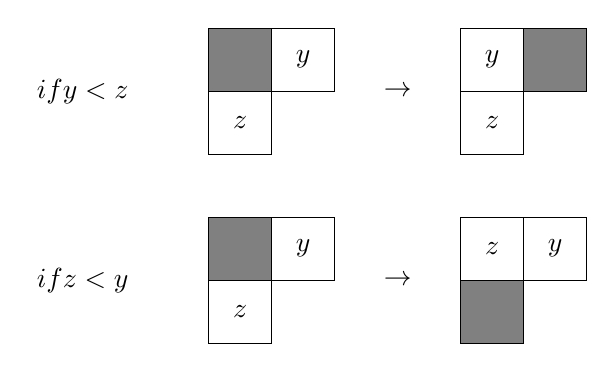
\begin{tikzpicture}
        \begin{scope}
          \node at (-1.6,-0.8) {$\text{if } y < z$};
          \draw[fill=gray] (0,0) rectangle ++(0.8,-0.8);
          \draw (0,0) rectangle ++(0.8,-0.8);
          \draw (0.8,0) rectangle ++(0.8,-0.8);
          \node at (1.2,-0.4) {$y$};
          \draw (0,-0.8) rectangle ++(0.8,-0.8);
          \node at (0.4,-1.2) {$z$};
          \node at (2.4,-0.8) {$\rightarrow $};

          \draw (3.2,0) rectangle ++(0.8,-0.8);
          \draw[fill=gray] (4,0) rectangle ++(0.8,-0.8);
          \draw (4,0) rectangle ++(0.8,-0.8);
          \node at (3.6,-0.4) {$y$};
          \draw (3.2,-0.8) rectangle ++(0.8,-0.8);
          \node at (3.6,-1.2) {$z$};
        \end{scope}
        \begin{scope}[yshift = -2.4cm]
          \node at (-1.6,-0.8) {$\text{if } z < y$};
          \draw[fill=gray] (0,0) rectangle ++(0.8,-0.8);
          \draw (0,0) rectangle ++(0.8,-0.8);
          \draw (0.8,0) rectangle ++(0.8,-0.8);
          \node at (1.2,-0.4) {$y$};
          \draw (0,-0.8) rectangle ++(0.8,-0.8);
          \node at (0.4,-1.2) {$z$};
          \node at (2.4,-0.8) {$\rightarrow $};

          \draw (3.2,0) rectangle ++(0.8,-0.8);
          \draw[fill=gray] (3.2,-0.8) rectangle ++(0.8,-0.8);
          \draw (4,0) rectangle ++(0.8,-0.8);
          \node at (4.4,-0.4) {$y$};
          \draw (3.2,-0.8) rectangle ++(0.8,-0.8);
          \node at (3.6,-0.4) {$z$};
        \end{scope}
      \end{tikzpicture}
    \end{figure}
  \end{defin}
\end{frame}

%19
\begin{frame}{edge labeled tableauxによる方法}
  \begin{block}{定義\ref{jeu de taquin}の続き}
  \begin{figure}
    \center
    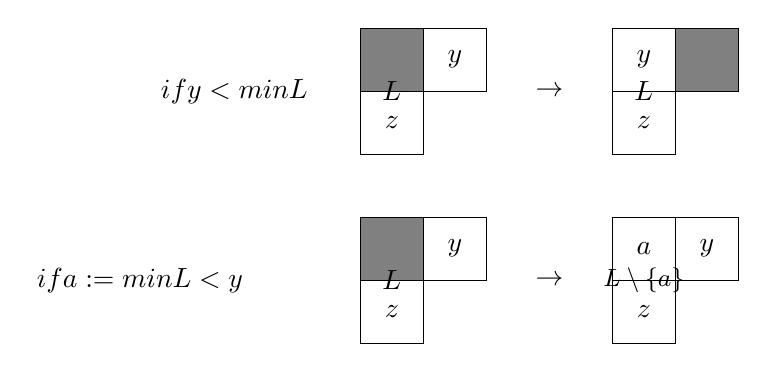
\begin{tikzpicture}
    \begin{scope}
      \node at (-1.6,-0.8) {$\text{if } y < \text{min }L$};
      \draw[fill=gray] (0,0) rectangle ++(0.8,-0.8);
      \node at (0.4,-0.8) {$L$};
      \draw (0,0) rectangle ++(0.8,-0.8);
      \draw (0.8,0) rectangle ++(0.8,-0.8);
      \node at (1.2,-0.4) {$y$};
      \draw (0,-0.8) rectangle ++(0.8,-0.8);
      \node at (0.4,-1.2) {$z$};
      \node at (2.4,-0.8) {$\rightarrow $};

      \draw (3.2,0) rectangle ++(0.8,-0.8);
      \draw[fill=gray] (4,0) rectangle ++(0.8,-0.8);
      \node at (3.6,-0.8) {$L$};
      \draw (4,0) rectangle ++(0.8,-0.8);
      \node at (3.6,-0.4) {$y$};
      \draw (3.2,-0.8) rectangle ++(0.8,-0.8);
      \node at (3.6,-1.2) {$z$};
    \end{scope}
    \begin{scope}[yshift = -2.4cm]
      \node at (-2.8,-0.8) {$\text{if } a:=\text{min }L < y$};
      \draw[fill=gray] (0,0) rectangle ++(0.8,-0.8);
      \node at (0.4,-0.8) {$L$};
      \draw (0,0) rectangle ++(0.8,-0.8);
      \draw (0.8,0) rectangle ++(0.8,-0.8);
      \node at (1.2,-0.4) {$y$};
      \draw (0,-0.8) rectangle ++(0.8,-0.8);
      \node at (0.4,-1.2) {$z$};
      \node at (2.4,-0.8) {$\rightarrow $};

      \draw (3.2,0) rectangle ++(0.8,-0.8);
      \node at (3.6,-0.4) {$a$};
      \node[font=\small] at (3.6,-0.8) {$L\setminus \{a\}$};
      \draw (4,0) rectangle ++(0.8,-0.8);
      \node at (4.4,-0.4) {$y$};
      \draw (3.2,-0.8) rectangle ++(0.8,-0.8);
      \node at (3.6,-1.2) {$z$};
    \end{scope}
  \end{tikzpicture}
  \end{figure}
  \end{block}
\end{frame}

%20
\begin{frame}{edge labeled tableauxによる方法}
  \begin{defin}
    $T\in\text{EqSYT}(\nu/\lambda,m)$に対して,次のような順番でequivariant jeu de taquinを施したtableauxをequivariant rectificationと呼び,$\text{EqRect}(T)$と書く.
    \begin{figure}
      \center
      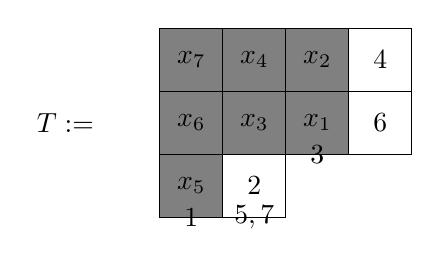
\begin{tikzpicture}
      \fill[gray] (0,0)--(2.4,0)--(2.4,-1.6)--(0.8,-1.6)--(0.8,-2.4)--(0,-2.4)--cycle;
        \draw (0,0)--(3.2,0)--(3.2,-1.6)--(1.6,-1.6)--(1.6,-2.4)--(0,-2.4)--cycle;
        \draw (0.8,0)-- +(0,-2.4);
        \draw (1.6,0)-- +(0,-1.6);
        \draw (2.4,0)-- +(0,-1.6);
        \draw (0,-0.8)-- +(3.2,0);
        \draw (0,-1.6)-- +(1.6,0);
  
        \node at (2.8,-0.4) {$4$};
        \node at (2.8,-1.2) {$6$};
        \node at (1.2,-2) {$2$};
        \node at (0.4,-2.4) {$1$};
        \node at (1.2,-2.4) {$5,7$};
        \node at (2,-1.6) {$3$};

        \node at (2,-1.2) {$x_1$};
        \node at (2,-0.4) {$x_2$};
        \node at (1.2,-1.2) {$x_3$};
        \node at (1.2,-0.4) {$x_4$};
        \node at (0.4,-2) {$x_5$};
        \node at (0.4,-1.2) {$x_6$};
        \node at (0.4,-0.4) {$x_7$};

        \node at (-1.2,-1.2) {$T:=$};
      \end{tikzpicture}
    \end{figure}
    に対して,
    \[
    \text{EqRect}(T) := \text{EqJdt}_{x_7}(\text{EqJdt}_{x_6}(\cdots\text{EqJdt}_{x_1}(T)))
    \]
  \end{defin}
\end{frame}

%21
\begin{frame}{edge labeled tableauxによる方法}
  \begin{eg}
    \begin{figure}[ht]
      \centering
      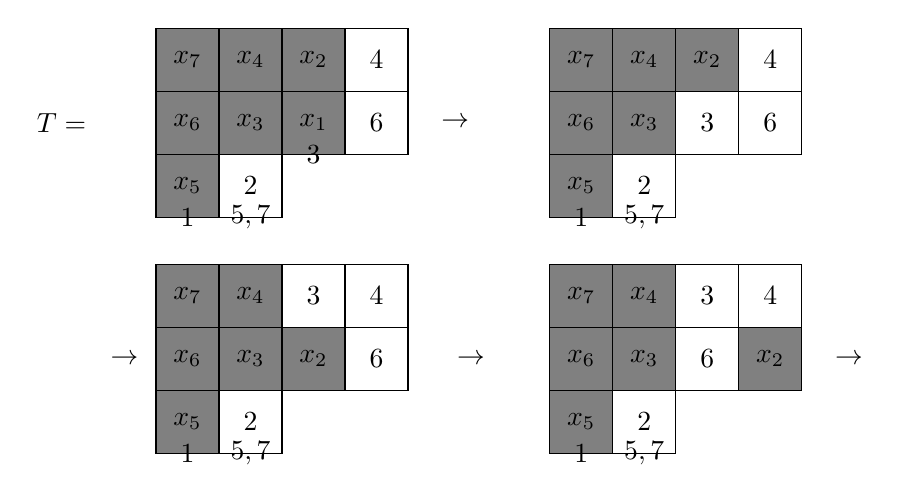
\begin{tikzpicture}
        \begin{scope}
          \fill[gray] (0,0)--(2.4,0)--(2.4,-1.6)--(0.8,-1.6)--(0.8,-2.4)--(0,-2.4)--cycle;
          \draw (0,0)--(3.2,0)--(3.2,-1.6)--(1.6,-1.6)--(1.6,-2.4)--(0,-2.4)--cycle;
          \draw (0.8,0)-- +(0,-2.4);
          \draw (1.6,0)-- +(0,-1.6);
          \draw (2.4,0)-- +(0,-1.6);
          \draw (0,-0.8)-- +(3.2,0);
          \draw (0,-1.6)-- +(1.6,0);
    
          \node at (2.8,-0.4) {$4$};
          \node at (2.8,-1.2) {$6$};
          \node at (1.2,-2) {$2$};
          \node at (0.4,-2.4) {$1$};
          \node at (1.2,-2.4) {$5,7$};
          \node at (2,-1.6) {$3$};
  
          \node at (2,-1.2) {$x_1$};
          \node at (2,-0.4) {$x_2$};
          \node at (1.2,-1.2) {$x_3$};
          \node at (1.2,-0.4) {$x_4$};
          \node at (0.4,-2) {$x_5$};
          \node at (0.4,-1.2) {$x_6$};
          \node at (0.4,-0.4) {$x_7$};
  
          \node at (-1.2,-1.2) {$T=$};
          \node at (3.8,-1.2) {$\rightarrow $};
        \end{scope}
        \begin{scope}[xshift=5cm]
          \fill[gray] (0,0)--(2.4,0)--(2.4,-0.8)--(1.6,-0.8)--(1.6,-1.6)--(0.8,-1.6)--(0.8,-2.4)--(0,-2.4)--cycle;
          \draw (0,0)--(3.2,0)--(3.2,-1.6)--(1.6,-1.6)--(1.6,-2.4)--(0,-2.4)--cycle;
          \draw (0.8,0)-- +(0,-2.4);
          \draw (1.6,0)-- +(0,-1.6);
          \draw (2.4,0)-- +(0,-1.6);
          \draw (0,-0.8)-- +(3.2,0);
          \draw (0,-1.6)-- +(1.6,0);
    
          \node at (2.8,-0.4) {$4$};
          \node at (2.8,-1.2) {$6$};
          \node at (1.2,-2) {$2$};
          \node at (0.4,-2.4) {$1$};
          \node at (1.2,-2.4) {$5,7$};
  
          \node at (2,-1.2) {$3$};
          \node at (2,-0.4) {$x_2$};
          \node at (1.2,-1.2) {$x_3$};
          \node at (1.2,-0.4) {$x_4$};
          \node at (0.4,-2) {$x_5$};
          \node at (0.4,-1.2) {$x_6$};
          \node at (0.4,-0.4) {$x_7$};
  
          
        \end{scope}
        \begin{scope}[yshift = -3cm]
          \node at (-0.4,-1.2) {$\rightarrow $};
          \fill[gray] (0,0)--(1.6,0)--(1.6,-1.6)--(0.8,-1.6)--(0.8,-2.4)--(0,-2.4)--cycle;
          \fill[gray] (1.6,-0.8) rectangle (2.4,-1.6);
          \draw (0,0)--(3.2,0)--(3.2,-1.6)--(1.6,-1.6)--(1.6,-2.4)--(0,-2.4)--cycle;
          \draw (0.8,0)-- +(0,-2.4);
          \draw (1.6,0)-- +(0,-1.6);
          \draw (2.4,0)-- +(0,-1.6);
          \draw (0,-0.8)-- +(3.2,0);
          \draw (0,-1.6)-- +(1.6,0);
    
          \node at (2.8,-0.4) {$4$};
          \node at (2.8,-1.2) {$6$};
          \node at (1.2,-2) {$2$};
          \node at (0.4,-2.4) {$1$};
          \node at (1.2,-2.4) {$5,7$};
  
          \node at (2,-1.2) {$x_2$};
          \node at (2,-0.4) {$3$};
          \node at (1.2,-1.2) {$x_3$};
          \node at (1.2,-0.4) {$x_4$};
          \node at (0.4,-2) {$x_5$};
          \node at (0.4,-1.2) {$x_6$};
          \node at (0.4,-0.4) {$x_7$};

          \node at (4,-1.2) {$\rightarrow$};
        \end{scope}

        \begin{scope}[xshift=5cm,yshift=-3cm]
          \fill[gray] (0,0)--(1.6,0)--(1.6,-1.6)--(0.8,-1.6)--(0.8,-2.4)--(0,-2.4)--cycle;
          \fill[gray] (2.4,-0.8) rectangle (3.2,-1.6);
          \draw (0,0)--(3.2,0)--(3.2,-1.6)--(1.6,-1.6)--(1.6,-2.4)--(0,-2.4)--cycle;
          \draw (0.8,0)-- +(0,-2.4);
          \draw (1.6,0)-- +(0,-1.6);
          \draw (2.4,0)-- +(0,-1.6);
          \draw (0,-0.8)-- +(3.2,0);
          \draw (0,-1.6)-- +(1.6,0);
    
          \node at (2.8,-0.4) {$4$};
          \node at (2.8,-1.2) {$x_2$};
          \node at (1.2,-2) {$2$};
          \node at (0.4,-2.4) {$1$};
          \node at (1.2,-2.4) {$5,7$};
  
          \node at (2,-1.2) {$6$};
          \node at (2,-0.4) {$3$};
          \node at (1.2,-1.2) {$x_3$};
          \node at (1.2,-0.4) {$x_4$};
          \node at (0.4,-2) {$x_5$};
          \node at (0.4,-1.2) {$x_6$};
          \node at (0.4,-0.4) {$x_7$};

          \node at (3.8,-1.2) {$\rightarrow $};
        \end{scope}
      \end{tikzpicture}
    \end{figure}
  \end{eg}
\end{frame}

%24
\begin{frame}{edge labeled tableauxによる方法}
  $T\in\text{EqSYT}(\nu/\lambda, m)$に対してもそのweightを定義することができ,
  \begin{theo}[Knutson-Tao]
    同変Littlewood-Richardson係数$C^\nu_{\lambda\mu}$について
    \[
    C^\nu_{\lambda\mu} = \sum_{\substack{
      T\in\text{EqSYT}(\nu/\lambda,|\mu|)\\
      \text{EqRect}(T) = T_\mu\\
      \text{wt}(T)\neq 0
    }}\text{wt}(T)
    \]
    が成り立つ.
    ここで$T_\mu$は形が$\mu$のstandard tableauxで,$1$行目から順に左から$1,2,\cdots,|\mu|$を書き入れたものである.
  \end{theo}
\end{frame}


\section[]{等価性}

%25
\begin{frame}{等価性}
  論文では紹介した2つの数え上げは本質的に同じであることを示した.すなわち,
  $\mathcal{P}^\nu_{\lambda\mu}=\set{P:\text{ puzzle}}{\partial P = \Delta^\nu_{\lambda\mu}}$,$\mathcal{T}^\nu_{\lambda\mu} = \set{T\in\text{EqSYT}(\nu/\lambda,|\mu|)}{\text{EqRect}(T)=T_\mu,\text{wt}(T)\neq 0}$としたとき,次を証明した.
  \begin{theo}\label{main theorem}
    全単射$\varphi:\mathcal{P}^\nu_{\lambda\mu}\rightarrow \mathcal{T}^\nu_{\lambda\mu}$であって$\text{wt}(\varphi(P))=\text{wt}(P)$を満たすものが存在する.
  \end{theo}
  定理\ref{main theorem}の$\varphi$は次のように構成できる.
\end{frame}

%26
\begin{frame}{等価性}
  \footnotesize
  puzzle $P$は一般に図のような形をしている.
  \begin{figure}
    \center
    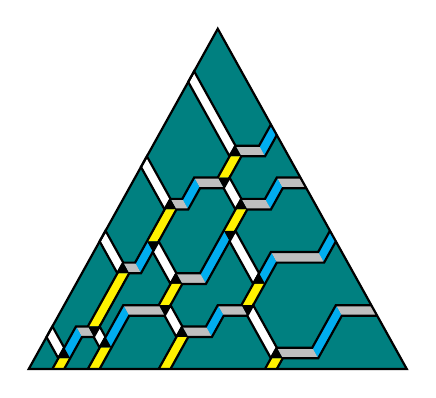
\begin{tikzpicture}[xscale = 0.3, yscale = 0.27, transform shape]
      \fill[teal] (0,0)--(16,0)--(8,16)--cycle;
  
  
  
      \fill[white] (3/4, 3/2)-- ++(2/4,-2/2)-- ++(1/4,1/2)-- ++(-2/4,2/2)--cycle;
      \draw[thick] (3/4, 3/2)-- ++(2/4,-2/2)-- ++(1/4,1/2)-- ++(-2/4,2/2)--cycle;
  
      \fill[white] (12/4, 12/2)-- ++(3/4,-3/2)-- ++(1/4,1/2)-- ++(-3/4,3/2)--cycle;
      \draw[thick] (12/4, 12/2)-- ++(3/4,-3/2)-- ++(1/4,1/2)-- ++(-3/4,3/2)--cycle;
  
      \fill[white] (19/4, 19/2)-- ++(4/4,-4/2)-- ++(1/4,1/2)-- ++(-4/4,4/2)--cycle;
      \draw[thick] (19/4, 19/2)-- ++(4/4,-4/2)-- ++(1/4,1/2)-- ++(-4/4,4/2)--cycle;
  
      \fill[white] (27/4, 27/2)-- ++(7/4,-7/2)-- ++(1/4,1/2)-- ++(-7/4,7/2)--cycle;
      \draw[thick] (27/4, 27/2)-- ++(7/4,-7/2)-- ++(1/4,1/2)-- ++(-7/4,7/2)--cycle;
  
      \fill[cyan] (8+9/4,16-9/2)-- ++(-2/4,-2/2)-- ++(1/4,-1/2)-- ++(2/4,2/2)--cycle;
      
      \fill[lightgray] (8+7/4,16-11/2)-- ++(-1,0)-- ++(1/4,-1/2)-- ++(1,0)--cycle;
      
      \fill[black] (8+3/4,16-11/2)-- ++(-1/4,-1/2)-- ++(1/2,0)--cycle;
      \fill[yellow] (8+2/4,16-12/2)-- ++(-2/4,-2/2)-- ++(1/2,0)-- ++(2/4,2/2)--cycle;
      
      \fill[black] (8,16-14/2)-- ++(1/2,0)-- ++(-1/4,-1/2)--cycle;
      \fill[lightgray] (8,16-14/2)-- ++(-1,0)-- ++(1/4,-1/2)-- ++(1,0)--cycle;
      
      \fill[cyan] (8-4/4,16-14/2)-- ++(-2/4,-2/2)-- ++(1/4,-1/2)-- ++(2/4,2/2)--cycle;
      
      \fill[lightgray] (8-6/4, 16-16/2)-- ++(-1/2,0)-- ++(1/4,-1/2)-- ++(1/2,0)--cycle;
      
      \fill[black] (8-8/4,16-16/2)-- ++(-1/4,-1/2)-- ++(1/2,0)--cycle;
      \fill[yellow] (8-9/4, 16-17/2)-- ++(-3/4,-3/2)-- ++(1/2,0)-- ++(3/4,3/2)--cycle;
      
      \fill[black] (8-12/4,16-20/2)-- ++(1/2,0)-- ++(-1/4,-1/2)--cycle;
      %
      \fill[cyan] (8-12/4,16-20/2)-- ++(-1/2,-2/2)-- ++(1/4,-1/2)-- ++(1/2,2/2)--cycle;
      
      \fill[lightgray] (8-14/4, 16-22/2)-- ++(-1/2,0)-- ++(1/4,-1/2)-- ++(1/2,0)--cycle;
      
      \fill[black] (8-16/4,16-22/2)-- ++(-1/4,-1/2)-- ++(1/2,0)--cycle;
      \fill[yellow] (8-17/4,16-23/2)-- ++(-5/4,-5/2)-- ++(1/2,0)-- ++(5/4,5/2)--cycle;
      
      \fill[black] (8-22/4,16-28/2)-- ++(1/2,0)-- ++(-1/4,-1/2)--cycle;
      \fill[lightgray] (8-22/4,16-28/2)-- ++(-1/2,0)-- ++(1/4,-1/2)-- ++(1/2,0)--cycle;
      
      \fill[cyan] (8-24/4,16-28/2)-- ++(-2/4,-2/2)-- ++(1/4,-1/2)-- ++(2/4,2/2)--cycle;
      
      \fill[black] (8-26/4,16-30/2)-- ++(-1/4,-1/2)-- ++(1/2,0)--cycle;
      \fill[yellow] (8-27/4, 16-31/2)-- ++(-1/4,-1/2)-- ++(1/2,0)-- ++(1/4,1/2)--cycle;
      
  
      \draw[thick] (8+9/4,16-9/2)-- ++(-1/2, -1)-- ++(-1,0)-- ++(-3/4, -3/2)-- ++(-1,0)-- ++(-1/2,-1)-- ++(-1/2,0)-- ++(-3/2,-3)-- ++(-1/2,0)-- ++(-3/2,-3)-- ++(-1/2,0)-- ++(-1,-2);
      \draw[thick] (8+10/4,16-5)-- ++(-1/2,-1)-- ++(-1,0)-- ++(-3/4,-3/2)-- ++(-1,0)-- ++(-1/2,-1)-- ++(-1/2,0)-- ++(-3/2,-3)-- ++(-1/2,0)-- ++(-3/2,-3)-- ++(-1/2, 0)-- ++(-3/4,-3/2);
  
  
  
      \fill[white] (8+4/4, 16-16/2)-- ++(-2/4,2/2)-- ++(-1/4,-1/2)-- ++(2/4,-2/2)--cycle;
      \draw[thick] (8+4/4, 16-16/2)-- ++(-2/4,2/2)-- ++(-1/4,-1/2)-- ++(2/4,-2/2)--cycle;
  
      \fill[white] (8-7/4,16-23/2)-- ++(-3/4,3/2)-- ++(-1/4,-1/2)-- ++(3/4,-3/2)--cycle;
      \draw[thick] (8-7/4,16-23/2)-- ++(-3/4,3/2)-- ++(-1/4,-1/2)-- ++(3/4,-3/2)--cycle;
  
      \fill[white] (8-19/4,16-29/2)-- ++(-1/4,1/2)-- ++(-1/4,-1/2)-- ++(1/4,-1/2)--cycle;
      \draw[thick] (8-19/4,16-29/2)-- ++(-1/4,1/2)-- ++(-1/4,-1/2)-- ++(1/4,-1/2)--cycle;
  
      \fill[lightgray] (8+14/4,16-14/2)-- ++(-1,0)-- ++(1/4,-1/2)-- ++(1,0)--cycle;
      
      \fill[cyan] (8+10/4,16-14/2)-- ++(-1/2,-1)-- ++(1/4,-1/2)-- ++(1/2,1)--cycle;
      
      \fill[lightgray] (8+8/4,16-16/2)-- ++(-1,0)-- ++(1/4,-1/2)-- ++(1,0)--cycle;
      
      \fill[black] (8+4/4, 16-16/2)-- ++(-1/4,-1/2)-- ++(1/2,0)--cycle;
      \fill[yellow] (8+3/4, 16-17/2)-- ++(-1/2,-1)-- ++(1/2,0)-- ++(1/2,1)--cycle;
      
      \fill[black] (8+1/4,16-19/2)-- ++(1/2,0)-- ++(-1/4,-1/2)--cycle;
      \fill[cyan] (8+1/4,16-19/2)-- ++(-1,-2)-- ++(1/4,-1/2)-- ++(1,2)--cycle;
      
      \fill[lightgray] (8-3/4,16-23/2)-- ++(-1,0)-- ++(1/4,-1/2)-- ++(1,0)--cycle;
      
      \fill[black] (8-7/4,16-23/2)-- ++(-1/4,-1/2)-- ++(1/2,0)--cycle;
      \fill[yellow] (8-8/4,16-24/2)-- ++(-1/2,-1)-- ++(1/2,0)-- ++(1/2,1)--cycle;
     
      \fill[black] (8-10/4,16-26/2)-- ++(1/2,0)-- ++(-1/4,-1/2)--cycle;
      \fill[lightgray] (8-10/4,16-26/2)-- ++(-3/2,0)-- ++(1/4,-1/2)-- ++(3/2,0)--cycle;
      
      \fill[cyan] (8-16/4,16-26/2)-- ++(-3/4,-3/2)-- ++(1/4,-1/2)-- ++(3/4,3/2)--cycle;
      
      \fill[black] (8-19/4,16-29/2)-- ++(-1/4,-1/2)-- ++(1/2,0)--cycle;
      \fill[yellow] (8-20/4,16-30/2)-- ++(-1/2,-1)-- ++(1/2,0)-- ++(1/2,1)--cycle;
      
  
      \draw[thick] (8+14/4,16-14/2)-- ++(-1,0)-- ++(-1/2,-1)-- ++(-1,0)-- ++(-7/4,-7/2)-- ++(-1,0)-- ++(-3/4,-3/2)-- ++(-3/2,0)-- ++(-6/4,-6/2);
      \draw[thick] (8+15/4, 16-15/2)-- ++(-1,0)-- ++(-1/2,-1)-- ++(-1,0)-- ++(-7/4,-7/2)-- ++(-1,0)-- ++(-3/4,-3/2)-- ++(-3/2,0)-- ++(-5/4,-5/2);
  
  
  
      \fill[white] (8+7/4,16-23/2)-- ++(-1,2)-- ++(-1/4,-1/2)-- ++(1,-2)--cycle;
      \draw[thick] (8+7/4,16-23/2)-- ++(-1,2)-- ++(-1/4,-1/2)-- ++(1,-2)--cycle;
  
      \fill[white] (8-6/4,16-28/2)-- ++(-1/2,1)-- ++(-1/4,-1/2)-- ++(1/2,-1)--cycle;
      \draw[thick] (8-6/4,16-28/2)-- ++(-1/2,1)-- ++(-1/4,-1/2)-- ++(1/2,-1)--cycle;
  
      \fill[cyan] (8+19/4,16-19/2)-- ++(-1/2,-1)-- ++(1/4,-1/2)-- ++(1/2,1)--cycle;
      
      \fill[lightgray] (8+17/4,16-21/2)-- ++(-2,0)-- ++(1/4,-1/2)-- ++(2,0)--cycle;
    
      \fill[cyan] (8+9/4,16-21/2)-- ++(-2/4,-2/2)-- ++(1/4,-1/2)-- ++(2/4,2/2)--cycle;
      
      \fill[black] (8+7/4,16-23/2)-- ++(-1/4,-1/2)-- ++(1/2,0)--cycle;
      \fill[yellow] (8+6/4,16-24/2)-- ++(-2/4,-2/2)-- ++(1/2,0)-- ++(1/2,1)--cycle;
  
      \fill[black] (8+4/4,16-26/2)-- ++(1/2,0)-- ++(-1/4,-1/2)--cycle;
      \fill[lightgray] (8+4/4,16-26/2)-- ++(-1,0)-- ++(1/4,-1/2)-- ++(1,0)--cycle;
      
      \fill[cyan] (8,16-26/2)-- ++(-1/2,-1)-- ++(1/4,-1/2)-- ++(1/2,1)--cycle;
  
      \fill[lightgray] (8-2/4,16-28/2)-- ++(-1,0)-- ++(1/4,-1/2)-- ++(1,0)--cycle;
      
      \fill[black] (8-6/4,16-28/2)-- ++(-1/4,-1/2)-- ++(1/2,0)--cycle;
      \fill[yellow] (8-7/4,16-29/2)-- ++(-3/4,-3/2)-- ++(1/2,0)-- ++(3/4,3/2)--cycle;

  
      \draw[thick] (8+19/4,16-19/2)-- ++(-1/2,-1)-- ++(-2,0)-- ++(-5/4,-5/2)-- ++(-1,0)-- ++(-1/2,-1)-- ++(-1,0)-- ++(-1,-2);
      \draw[thick] (8+20/4,16-20/2)-- ++(-1/2,-1)-- ++(-2,0)-- ++(-5/4,-5/2)-- ++(-1,0)-- ++(-1/2,-1)-- ++(-1,0)-- ++(-3/4,-3/2);
  
  
  
      \fill[white] (8+10/4,16-30/2)-- ++(-1,2)-- ++(-1/4,-1/2)-- ++(1,-2)--cycle;
      \draw[thick] (8+10/4,16-30/2)-- ++(-1,2)-- ++(-1/4,-1/2)-- ++(1,-2)--cycle;
  
      \fill[lightgray] (8+26/4, 16-26/2)-- ++(-3/2,0)-- ++(1/4,-1/2)-- ++(3/2,0)--cycle;

      \fill[cyan] (8+20/4, 16-26/2)-- ++(-1,-2)-- ++(1/4,-1/2)-- ++(1,2)--cycle;

      \fill[lightgray] (8+16/4,16-30/2)-- ++(-3/2,0)-- ++(1/4,-1/2)-- ++(3/2,0)--cycle;

      \fill[black] (8+10/4,16-30/2)-- ++(-1/4,-1/2)-- ++(1/2,0)--cycle;
      \fill[yellow] (8+9/4,16-31/2)-- ++(-1/4,-1/2)-- ++(1/2,0)-- ++(1/4,1/2)--cycle;

  
      \draw[thick] (8+26/4, 16-26/2)-- ++(-3/2,0)-- ++(-1,-2)-- ++(-3/2,0)-- ++(-1/2,-1);
      \draw[thick] (8+27/4, 16-27/2)-- ++(-3/2,0)-- ++(-1,-2)-- ++(-3/2,0)-- ++(-1/4,-1/2);
  
      \draw[thick] (0,0)--(16,0)--(8,16)--cycle;
    \end{tikzpicture}
  \end{figure}
  ただし,ラベルを表示する代わりに,各pieceに異なる色をつけて表している.
  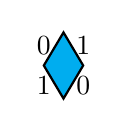
\begin{tikzpicture}[baseline=-1pt][xscale=0.7,yscale=0.7]
    \fill[cyan] (0,0)--(0.25,0.42)--(0.5,0)--(0.25,-0.42)--cycle;
    \protect\draw[thick] (0,0)--(0.25,0.42)--(0.5,0)--(0.25,-0.42)--cycle;
    \protect\node at (0,0.25) {$0$};
    \protect\node at (0.5,0.25) {$1$};
    \protect\node at (0,-0.25) {$1$};
    \protect\node at (0.5,-0.25) {$0$};
  \end{tikzpicture}
  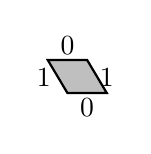
\begin{tikzpicture}[baseline=2pt][xscale=0.7,yscale=0.7]
    \fill[lightgray] (0,0)-- ++(0.5,0)-- ++(-0.25,0.42)-- ++(-0.5,0)--cycle;
    \protect\draw[thick](0,0)-- ++(0.5,0)-- ++(-0.25,0.42)-- ++(-0.5,0)--cycle;
    \protect\node at (-0.3,0.2) {$1$};
    \protect\node at (0.25,-0.18) {$0$};
    \protect\node at (0.5,0.2) {$1$};
    \protect\node at (0, 0.6) {$0$};
  \end{tikzpicture}
  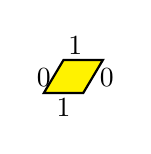
\begin{tikzpicture}[baseline=2pt][xscale=0.7,yscale=0.7]
    \fill[yellow] (0,0)-- ++(0.5,0)-- ++(0.25,0.42)-- ++(-0.5,0)--cycle;
    \protect\draw[thick](0,0)-- ++(0.5,0)-- ++(0.25,0.42)-- ++(-0.5,0)--cycle;
    \protect\node at (0,0.2) {$0$};
    \protect\node at (0.25,-0.18) {$1$};
    \protect\node at (0.8,0.2) {$0$};
    \protect\node at (0.4, 0.6) {$1$};
  \end{tikzpicture}
  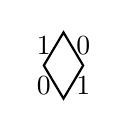
\begin{tikzpicture}[baseline=-1pt][xscale=0.7,yscale=0.7]
    \protect\draw[thick] (0,0)--(0.25,0.42)--(0.5,0)--(0.25,-0.42)--cycle;
    \protect\node at (0,0.25) {$1$};
    \protect\node at (0.5,0.25) {$0$};
    \protect\node at (0,-0.25) {$0$};
    \protect\node at (0.5,-0.25) {$1$};
  \end{tikzpicture}
  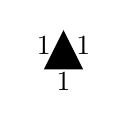
\begin{tikzpicture}[baseline=1pt][xscale=0.7,yscale=0.7]
    \fill[black] (0,0)-- ++(0.5,0)-- ++(-0.25,0.5)--cycle;
    \protect\node at (0,0.3) {$1$};
    \protect\node at (0.5,0.3) {$1$};
    \protect\node at (0.25,-0.15) {$1$};
  \end{tikzpicture}
  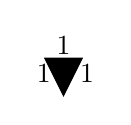
\begin{tikzpicture}[baseline=2pt][xscale=0.7,yscale=0.7]
    \fill[black] (0,0.5)-- ++(0.5,0)-- ++(-0.25,-0.5)--cycle;
    \protect\node at (0.25, 0.65) {$1$};
    \protect\node at (0,0.3) {$1$};
    \protect\node at (0.55,0.3) {$1$};
  \end{tikzpicture}
  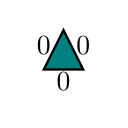
\begin{tikzpicture}[baseline=1pt][xscale=0.7,yscale=0.7]
    \fill[teal] (0,0)-- ++(0.5,0)-- ++(-0.25,0.5)--cycle;
    \protect\draw[thick] (0,0)-- ++(0.5,0)-- ++(-0.25,0.5)--cycle;
    \protect\node at (0,0.3) {$0$};
    \protect\node at (0.5,0.3) {$0$};
    \protect\node at (0.25,-0.15) {$0$};
  \end{tikzpicture}
  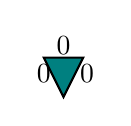
\begin{tikzpicture}[baseline=2pt][xscale=0.7,yscale=0.7]
    \fill[teal] (0,0.5)-- ++(0.5,0)-- ++(-0.25,-0.5)--cycle;
    \protect\draw[thick] (0,0.5)-- ++(0.5,0)-- ++(-0.25,-0.5)--cycle;
    \protect\node at (0.25, 0.65) {$0$};
    \protect\node at (0,0.3) {$0$};
    \protect\node at (0.55,0.3) {$0$};
  \end{tikzpicture}
  \normalsize
\end{frame}

%27
\begin{frame}{等価性}
  
\begin{tikzpicture}[baseline=-1pt]
    \fill[cyan] (0,0)--(0.25,0.42)--(0.5,0)--(0.25,-0.42)--cycle;
    \draw[thick] (0,0)--(0.25,0.42)--(0.5,0)--(0.25,-0.42)--cycle;
  \end{tikzpicture}
  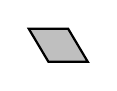
\begin{tikzpicture}[baseline=2pt]
    \fill[lightgray] (0,0)-- ++(0.5,0)-- ++(-0.25,0.42)-- ++(-0.5,0)--cycle;
    \draw[thick](0,0)-- ++(0.5,0)-- ++(-0.25,0.42)-- ++(-0.5,0)--cycle;
  \end{tikzpicture}
  
\begin{tikzpicture}[baseline=2pt]
    \fill[yellow] (0,0)-- ++(0.5,0)-- ++(0.25,0.42)-- ++(-0.5,0)--cycle;
    \draw[thick](0,0)-- ++(0.5,0)-- ++(0.25,0.42)-- ++(-0.5,0)--cycle;
  \end{tikzpicture}
  
\begin{tikzpicture}[baseline=1pt]
    \fill[black] (0,0)-- ++(0.5,0)-- ++(-0.25,0.5)--cycle;
  \end{tikzpicture}
  
\begin{tikzpicture}[baseline=2pt]
    \fill[black] (0,0.5)-- ++(0.5,0)-- ++(-0.25,-0.5)--cycle;
  \end{tikzpicture}
  のpuzzle pieceからなる連結領域をpath と呼び,
  
\begin{tikzpicture}[baseline=2pt]
    \fill[black] (0,0.5)-- ++(0.5,0)-- ++(-0.25,-0.5)--cycle;
  \end{tikzpicture}
  で挟まれた部分をsegmentと呼ぶ.

  \begin{figure}
    \center
    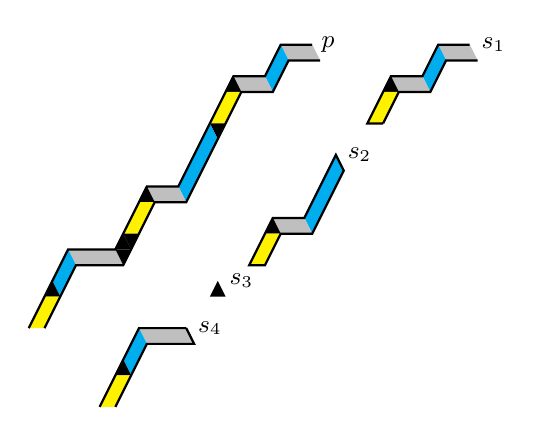
\begin{tikzpicture}[xscale = 0.4,yscale = 0.4]
      \node[font=\small] at (8+16/4,16-14/2) {$p$};
      \fill[lightgray] (8+14/4,16-14/2)-- ++(-1,0)-- ++(1/4,-1/2)-- ++(1,0)--cycle;
      \fill[cyan] (8+10/4,16-14/2)-- ++(-1/2,-1)-- ++(1/4,-1/2)-- ++(1/2,1)--cycle;
      \fill[lightgray] (8+8/4,16-16/2)-- ++(-1,0)-- ++(1/4,-1/2)-- ++(1,0)--cycle;
      \fill[black] (8+4/4, 16-16/2)-- ++(-1/4,-1/2)-- ++(1/2,0)--cycle;
      \fill[yellow] (8+3/4, 16-17/2)-- ++(-1/2,-1)-- ++(1/2,0)-- ++(1/2,1)--cycle;
      \fill[black] (8+1/4,16-19/2)-- ++(1/2,0)-- ++(-1/4,-1/2)--cycle;
      \fill[cyan] (8+1/4,16-19/2)-- ++(-1,-2)-- ++(1/4,-1/2)-- ++(1,2)--cycle;
      \fill[lightgray] (8-3/4,16-23/2)-- ++(-1,0)-- ++(1/4,-1/2)-- ++(1,0)--cycle;
      \fill[black] (8-7/4,16-23/2)-- ++(-1/4,-1/2)-- ++(1/2,0)--cycle;
      \fill[yellow] (8-8/4,16-24/2)-- ++(-1/2,-1)-- ++(1/2,0)-- ++(1/2,1)--cycle;
      \fill[black] (8-10/4,16-26/2)-- ++(1/2,0)-- ++(-1/4,-1/2)--cycle;
      \fill[lightgray] (8-11/4,16-27/2)-- ++(-3/2,0)-- ++(1/4,-1/2)-- ++(3/2,0)--cycle;
      \fill[black] (8-10/4,16-26/2)-- ++(-1/4,-1/2)-- ++(1/2,0)--cycle;
      \fill[black] (8-9/4,16-27/2)-- ++(-1/2,0)-- ++(1/4,-1/2)--cycle;
      \fill[cyan] (8-17/4,16-27/2)-- ++(-2/4,-2/2)-- ++(1/4,-1/2)-- ++(2/4,2/2)--cycle;
      \fill[black] (8-19/4,16-29/2)-- ++(-1/4,-1/2)-- ++(1/2,0)--cycle;
      \fill[yellow] (8-20/4,16-30/2)-- ++(-1/2,-1)-- ++(1/2,0)-- ++(1/2,1)--cycle;
  
  
      \draw[thick] (8+14/4,16-14/2)-- ++(-1,0)-- ++(-1/2,-1)-- ++(-1,0)-- ++(-7/4,-7/2)-- ++(-1,0)-- ++(-4/4,-4/2)-- ++(-3/2,0)-- ++(-5/4,-5/2);
      \draw[thick] (8+15/4, 16-15/2)-- ++(-1,0)-- ++(-1/2,-1)-- ++(-1,0)-- ++(-7/4,-7/2)-- ++(-1,0)-- ++(-4/4,-4/2)-- ++(-3/2,0)-- ++(-4/4,-4/2);
  
      \begin{scope}[xshift=5cm]
      \node[font=\small] at (8+17/4,16-14/2) {$s_1$};
      \fill[lightgray] (8+14/4,16-14/2)-- ++(-1,0)-- ++(1/4,-1/2)-- ++(1,0)--cycle;
      \fill[cyan] (8+10/4,16-14/2)-- ++(-1/2,-1)-- ++(1/4,-1/2)-- ++(1/2,1)--cycle;
      \fill[lightgray] (8+8/4,16-16/2)-- ++(-1,0)-- ++(1/4,-1/2)-- ++(1,0)--cycle;
      \fill[black] (8+4/4, 16-16/2)-- ++(-1/4,-1/2)-- ++(1/2,0)--cycle;
      \fill[yellow] (8+3/4, 16-17/2)-- ++(-1/2,-1)-- ++(1/2,0)-- ++(1/2,1)--cycle;
      
      \draw[thick] (8+14/4,16-14/2)-- ++(-1,0)-- ++(-1/2,-1)-- ++(-1,0)-- ++(-3/4,-3/2)-- ++(1/2,0);
      \draw[thick] (8+15/4, 16-15/2)-- ++(-1,0)-- ++(-1/2,-1)-- ++(-1,0)-- ++(-2/4,-2/2);
      \end{scope}
  
      \begin{scope}[xshift=4cm, yshift=-1cm]
      \node[font=\small] at (8+4/4,16-19/2) {$s_2$};
      \fill[cyan] (8+1/4,16-19/2)-- ++(-1,-2)-- ++(1/4,-1/2)-- ++(1,2)--cycle;
      \fill[lightgray] (8-3/4,16-23/2)-- ++(-1,0)-- ++(1/4,-1/2)-- ++(1,0)--cycle;
      \fill[black] (8-7/4,16-23/2)-- ++(-1/4,-1/2)-- ++(1/2,0)--cycle;
      \fill[yellow] (8-8/4,16-24/2)-- ++(-1/2,-1)-- ++(1/2,0)-- ++(1/2,1)--cycle;
  
      \draw[thick] (8+1/4,16-19/2)-- ++(-1,-2)-- ++(-1,0)-- ++(-3/4,-3/2)-- ++(1/2,0)-- ++(2/4,2/2)-- ++(1,0)-- ++(1,2)--cycle;
      \end{scope}
  
      \begin{scope}[xshift=3cm, yshift=-1.5cm]
        \fill[black] (8-10/4,16-26/2)-- ++(-1/4,-1/2)-- ++(1/2,0)--cycle;
        \node[font=\small] at (8-7/4,16-26/2) {$s_3$};
      \end{scope}
  
      \begin{scope}[xshift=2cm, yshift=-3cm]
        \node[font=\small] at(8-7/4,16-26/2) {$s_4$};
        \fill[lightgray] (8-10/4,16-26/2)-- ++(-3/2,0)-- ++(1/4,-1/2)-- ++(3/2,0)--cycle;
      \fill[cyan] (8-16/4,16-26/2)-- ++(-2/4,-2/2)-- ++(1/4,-1/2)-- ++(2/4,2/2)--cycle;
      \fill[black] (8-18/4,16-28/2)-- ++(-1/4,-1/2)-- ++(1/2,0)--cycle;
      \fill[yellow] (8-19/4,16-29/2)-- ++(-1/2,-1)-- ++(1/2,0)-- ++(1/2,1)--cycle;
  
      \draw[thick] (8-10/4,16-26/2)-- ++(-3/2,0)-- ++(-5/4,-5/2);
      \draw[thick] (8-10/4,16-26/2)-- ++(1/4,-1/2)-- ++(-1.5,0)-- ++(-4/4,-4/2);
      \end{scope}
    \end{tikzpicture}
  \end{figure}
\end{frame}

%28
\begin{frame}{等価性}
  $\Lambda = ((n-k)^k)$とする.$P$のpathを$p_1,\cdots,p_k$として,$p_1$から順に次のような操作を行って$\Lambda$の箱と辺にラベルを書き入れて得られるtableauxを$\varphi(P)$とする.
  \begin{eg}\label{algorithm example}
    \begin{figure}
      \begin{tikzpicture}[xscale = 0.5, yscale = 0.5]
        \center
        \fill[teal] (0,0)-- ++(8,0)-- ++(-4,8)--cycle;
        \draw (0,0)-- ++(8,0)-- ++(-4,8)--cycle;
    
        \fill[black] (2,2)--++(1,0)--++(1/2,1)-- ++(-1/2,1)--++(-1,0)-- ++(-1/2,-1)-- ++(-1/2,-1);
        \fill[black] (1/2,1)-- ++(1,0)-- ++(-1/2,1)--cycle;
        \fill[black] (2.5, 5)-- ++(1,0)-- ++(-1/2,1)--cycle;
        \fill[black] (4,2)-- ++(1/2,-1)-- ++(-1,0)--cycle;
    
        \foreach \x in {1,...,7}{
          \draw[gray,thick] (\x, 0) -- (\x/2, \x);
          \draw[gray,thick] (\x, 0) -- (4+\x/2, 8-\x);
          \draw[gray,thick] (\x/2,\x) -- (8-\x/2,\x);
        };
        
        \fill[yellow] (0,0)-- ++(1,0)-- ++(1/2,1)--++(-1,0)--cycle;
        \draw[gray,thick](0,0)-- ++(1,0)-- ++(1/2,1)--++(-1,0)--cycle;
        \fill[cyan] (3/2,1)-- ++(1/2,1)-- ++(-1/2,1)-- ++(-1/2,-1);
        \draw[gray,thick](3/2,1)-- ++(1/2,1)-- ++(-1/2,1)-- ++(-1/2,-1);
        \fill[yellow] (2,4)-- ++(1,0)-- ++(1/2,1)-- ++(-1,0)--cycle;
        \draw[gray,thick](2,4)-- ++(1,0)-- ++(1/2,1)-- ++(-1,0)--cycle;
        \fill[lightgray] (3,6)-- ++(1,0)-- ++(1/2,-1)-- ++(-1,0)--cycle;
        \draw[gray,thick](3,6)-- ++(1,0)-- ++(1/2,-1)-- ++(-1,0)--cycle;
        \fill[cyan] (4,6)-- ++(1/2,-1)-- ++(1/2,1)-- ++(-1/2,1)--cycle;
        \draw[gray,thick](4,6)-- ++(1/2,-1)-- ++(1/2,1)-- ++(-1/2,1)--cycle;
        \fill[yellow] (1,0)-- ++(1,0)-- ++(1/2,1)--++(-1,0)--cycle;
        \draw[gray,thick](1,0)-- ++(1,0)-- ++(1/2,1)--++(-1,0)--cycle;
        \fill[yellow] (3/2,1)-- ++(1,0)-- ++(1/2,1)--++(-1,0)--cycle;
        \draw[gray,thick](3/2,1)-- ++(1,0)-- ++(1/2,1)--++(-1,0)--cycle;
    
        \fill[lightgray](3,4)-- ++(1,0)-- ++(1/2,-1)-- ++(-1,0)--cycle;
        \draw[gray,thick](3,4)-- ++(1,0)-- ++(1/2,-1)-- ++(-1,0)--cycle;
    
        \fill[lightgray](4,4)-- ++(1,0)-- ++(1/2,-1)-- ++(-1,0)--cycle;
        \draw[gray,thick](4,4)-- ++(1,0)-- ++(1/2,-1)-- ++(-1,0)--cycle;
    
        \fill[lightgray](5,4)-- ++(1,0)-- ++(1/2,-1)-- ++(-1,0)--cycle;
        \draw[gray,thick](5,4)-- ++(1,0)-- ++(1/2,-1)-- ++(-1,0)--cycle;
    
        \fill[white] (3,2)-- ++(1/2,1)-- ++(1/2,-1)-- ++(-1/2,-1)--cycle;
        \draw[gray,thick](3,2)-- ++(1/2,1)-- ++(1/2,-1)-- ++(-1/2,-1)--cycle;
    
        \fill[yellow] (3,0)-- ++(1,0)-- ++(1/2,1)--++(-1,0)--cycle;
        \draw[thick,gray] (3,0)-- ++(1,0)-- ++(1/2,1)--++(-1,0)--cycle;
    
        \fill[lightgray] (4,2)-- ++(1,0)-- ++(1/2,-1)-- ++(-1,0)--cycle;
        \draw[gray, thick] (4,2)-- ++(1,0)-- ++(1/2,-1)-- ++(-1,0)--cycle;
    
        \fill[lightgray] (5,2)-- ++(1,0)-- ++(1/2,-1)-- ++(-1,0)--cycle;
        \draw[gray, thick] (5,2)-- ++(1,0)-- ++(1/2,-1)-- ++(-1,0)--cycle;
    
        \fill[cyan] (6,2)-- ++(1/2,-1)-- ++(1/2,1)-- ++(-1/2,1)--cycle;
        \draw[gray,thick] (6,2)-- ++(1/2,-1)-- ++(1/2,1)-- ++(-1/2,1)--cycle;
      \end{tikzpicture}
    \end{figure}
    図のpuzzle $P\in \mathcal{P}^{01010100}_{01001100,11010000}$を用いて説明する.
  \end{eg}
\end{frame}

%29
\begin{frame}{等価性}
  \begin{exampleblock}{例\ref{algorithm example}の続き}
    $P$のpathは
    \begin{figure}
      \center
      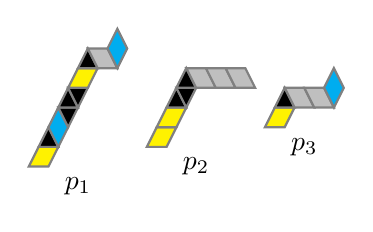
\begin{tikzpicture}[xscale = 0.5, yscale = 0.5]
        \begin{scope}
          \node at (5/4, -1/2) {$p_1$};
          \fill[yellow] (0,0)-- ++(1/2,0)-- ++(1/4,1/2)-- ++(-1/2,0)--cycle;
          \draw[thick,gray] (0,0)-- ++(1/2,0)-- ++(1/4,1/2)-- ++(-1/2,0)--cycle;
    
          \filldraw[fill=black, draw=gray,thick] (1/4,1/2)-- ++(1/2,0)-- ++(-1/4,1/2)--cycle;
    
          \filldraw[fill=cyan, draw=gray,thick] (1/2,1)-- ++(1/4,-1/2)-- ++(1/4,1/2)-- ++(-1/4,1/2)--cycle;
    
          \fill[black] (1,1)-- ++(1/4,1/2)-- ++(-1/2,0)--cycle;
          \draw[thick,gray] (1,1)-- ++(1/4,1/2)-- ++(-1/2,0)--cycle;
    
          \fill[black] (3/4,1+1/2)-- ++(1/2,0)-- ++(-1/4,1/2)--cycle;
          \draw[thick,gray] (3/4,1+1/2)-- ++(1/2,0)-- ++(-1/4,1/2)--cycle;
    
          \fill[black] (1+1/4,1+1/2)-- ++(1/4,1/2)-- ++(-1/2,0)--cycle;
          \draw[thick,gray] (1+1/4,1+1/2)-- ++(1/4,1/2)-- ++(-1/2,0)--cycle;
    
          \filldraw[fill=yellow, draw=gray,thick] (1,2)-- ++(1/2,0)-- ++(1/4,1/2)-- ++(-1/2,0)--cycle;
    
          \filldraw[fill=black, draw=gray,thick] (5/4,5/2)-- ++(1/2,0)-- ++(-1/4,1/2)--cycle;
    
          \filldraw[fill=lightgray, draw=gray,thick] (6/4,6/2)-- ++(1/2,0)-- ++(1/4,-1/2)-- ++(-1/2,0)--cycle;
    
          \filldraw[fill=cyan, draw=gray,thick] (8/4,6/2)-- ++(1/4,-1/2)-- ++(1/4,1/2)-- ++(-1/4,1/2)--cycle;
        \end{scope}
        \begin{scope}[xshift=3cm, yshift=0.5cm]
          \node at (5/4, -1/2) {$p_2$};
          \filldraw[fill=yellow, draw=gray,thick] (0,0)-- ++(1/2,0)-- ++(1/4,1/2)-- ++(-1/2,0)--cycle;
          \filldraw[fill=yellow, draw=gray,thick] (1/4,1/2)-- ++(1/2,0)-- ++(1/4,1/2)-- ++(-1/2,0)--cycle;
          \filldraw[fill=black, draw=gray,thick] (1/2,1)-- ++(1/2,0)-- ++(-1/4,1/2)--cycle;
          %
          \filldraw[fill=black, draw=gray,thick] (3/4,3/2)-- ++(1/2,0)-- ++(-1/4,-1/2)--cycle;
          \filldraw[fill=black, draw=gray,thick] (3/4,3/2)-- ++(1/2,0)-- ++(-1/4,1/2)--cycle;
          \filldraw[fill=lightgray, draw=gray,thick] (4/4,4/2)-- ++(1/2,0)-- ++(1/4,-1/2)-- ++(-1/2,0)--cycle;
          \filldraw[fill=lightgray, draw=gray,thick] (6/4,4/2)-- ++(1/2,0)-- ++(1/4,-1/2)-- ++(-1/2,0)--cycle;
          \filldraw[fill=lightgray, draw=gray,thick] (8/4,4/2)-- ++(1/2,0)-- ++(1/4,-1/2)-- ++(-1/2,0)--cycle;
        \end{scope}
        \begin{scope}[xshift=6cm, yshift=1cm]
          \node at (4/4, -1/2) {$p_3$};
          \filldraw[fill=yellow, draw=gray,thick] (0,0)-- ++(1/2,0)-- ++(1/4,1/2)-- ++(-1/2,0)--cycle;
          \filldraw[fill=black, draw=gray,thick] (1/4,1/2)-- ++(1/2,0)-- ++(-1/4,1/2)--cycle;
          \filldraw[fill=lightgray, draw=gray,thick] (2/4,2/2)-- ++(1/2,0)-- ++(1/4,-1/2)-- ++(-1/2,0)--cycle;
          \filldraw[fill=lightgray, draw=gray,thick] (4/4,2/2)-- ++(1/2,0)-- ++(1/4,-1/2)-- ++(-1/2,0)--cycle;
          \filldraw[fill=cyan, draw=gray,thick] (6/4,2/2)-- ++(1/4,-1/2)-- ++(1/4,1/2)-- ++(-1/4,1/2)--cycle;
        \end{scope}
      \end{tikzpicture}
    \end{figure}
    であり,$p_1$から順に以下の図のようにラベルを書き入れる
    \begin{figure}
      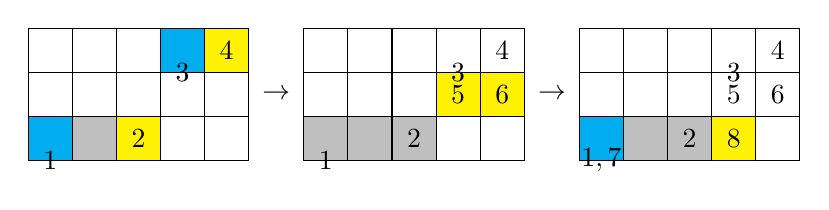
\begin{tikzpicture}[xscale = 0.7, yscale = 0.7]
        \begin{scope}
          \fill[cyan] (0,0) rectangle ++(0.8,0.8);
          \fill[lightgray] (0.8,0) rectangle ++(0.8,0.8);
          \fill[yellow] (1.6,0) rectangle ++(0.8,0.8);
  
          \fill[cyan] (2.4,1.6) rectangle ++(0.8,0.8);
          \fill[yellow] (3.2,1.6) rectangle ++(0.8,0.8);
  
          \draw (0,0) rectangle (4, 2.4);
          \foreach \x in {1,...,4} {
            \draw (\x * 0.8, 0) -- (\x * 0.8, 2.4);
          };
          \foreach \x in {1,2} {
            \draw (0, \x * 0.8) -- (4, \x * 0.8);
          };
  
          \node at (0.4,0) {$1$};
          \node at (2, 0.4) {$2$};
          \node at (2.8, 1.6) {$3$};
          \node at (3.6, 2) {$4$};
          
          \node at (4.5, 1.2) {$\rightarrow$};
        \end{scope}
        \begin{scope}[xshift=5cm]
          \fill[lightgray] (0,0) rectangle ++(0.8,0.8);
          \fill[lightgray] (0.8,0) rectangle ++(0.8,0.8);
          \fill[lightgray] (1.6,0) rectangle ++(0.8,0.8);
  
          \fill[yellow] (2.4,0.8) rectangle ++(0.8,0.8);
          \fill[yellow] (3.2,0.8) rectangle ++(0.8,0.8);
  
          \draw (0,0) rectangle (4, 2.4);
          \foreach \x in {1,...,4} {
            \draw (\x * 0.8, 0) -- (\x * 0.8, 2.4);
          };
          \foreach \x in {1,2} {
            \draw (0, \x * 0.8) -- (4, \x * 0.8);
          };
  
          \node at (0.4,0) {$1$};
          \node at (2, 0.4) {$2$};
          \node at (2.8, 1.6) {$3$};
          \node at (3.6, 2) {$4$};
          \node at (2.8,1.2) {$5$};
          \node at (3.6,1.2) {$6$};
  
          \node at (4.5, 1.2) {$\rightarrow$};
        \end{scope}
        \begin{scope}[xshift=10cm]
          \fill[cyan] (0,0) rectangle ++(0.8,0.8);
          \fill[lightgray] (0.8,0) rectangle ++(0.8,0.8);
          \fill[lightgray] (1.6,0) rectangle ++(0.8,0.8);
          \fill[yellow] (2.4,0) rectangle ++(0.8,0.8);
  
          \draw (0,0) rectangle (4, 2.4);
          \foreach \x in {1,...,4} {
            \draw (\x * 0.8, 0) -- (\x * 0.8, 2.4);
          };
          \foreach \x in {1,2} {
            \draw (0, \x * 0.8) -- (4, \x * 0.8);
          };
  
          \node at (0.4,0) {$1,7$};
          \node at (2, 0.4) {$2$};
          \node at (2.8, 1.6) {$3$};
          \node at (3.6, 2) {$4$};
          \node at (2.8,1.2) {$5$};
          \node at (3.6,1.2) {$6$};
          \node at (2.8,0.4) {$8$};
        \end{scope}
      \end{tikzpicture}
    \end{figure}
  \end{exampleblock}
\end{frame}

%30
\begin{frame}{等価性}
  \begin{exampleblock}{例\ref{algorithm example}の続き}
    処理を行った箱すべてを含む領域の左上の部分を$\varphi(P)$とする.
    \begin{figure}
      \center
      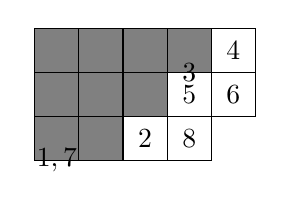
\begin{tikzpicture}[xscale = 0.7, yscale = 0.7]
        \fill[gray] (0,0)-- ++(3.2,0)-- ++(0,-0.8)-- ++(-0.8,0)-- ++(0,-0.8)-- ++(-0.8,0)-- ++(0,-0.8)-- ++(-1.6,0)--cycle;
        \draw (0,0)-- ++(4,0)-- ++(0,-1.6)-- ++(-0.8,0)-- ++(0,-0.8)-- ++(-3.2,0)--cycle;
        \draw (0.8,0) -- ++(0,-2.4);
        \draw (1.6,0) -- ++(0,-2.4);
        \draw (2.4,0) -- ++(0,-2.4);
        \draw (3.2,0) -- ++(0,-2.4);
        \draw (0,-0.8) -- ++(4,0);
        \draw (0,-1.6) -- ++(4,0);
  
        \node at (0.4,-2.4) {$1,7$};
          \node at (2, -2) {$2$};
          \node at (2.8, -0.8) {$3$};
          \node at (3.6, -0.4) {$4$};
          \node at (2.8,-1.2) {$5$};
          \node at (3.6,-1.2) {$6$};
          \node at (2.8,-2) {$8$};
      \end{tikzpicture}
    \end{figure}
  \end{exampleblock}
\end{frame}


\end{document}